\documentclass[a4paper, 10pt]{article}
\usepackage[utf8]{inputenc}
\usepackage[english,russian]{babel}
\usepackage{fancyhdr}
\usepackage{caption}
\usepackage[left=1.5cm,right=1.5cm,top=2cm,bottom=1.5cm,bindingoffset=0cm]{geometry}
\captionsetup{labelsep=period}
\pagestyle{fancy}
\usepackage{listings,longtable,amsmath,amsfonts,graphicx,tikz,tabularx}
\usepackage{float}

\lstset{
    basicstyle=\footnotesize,
    breakatwhitespace=false,
    breaklines=true,
    extendedchars=true,
    keepspaces=true,
    keywordstyle=\bfseries,
    numbers=left,
    numbersep=3pt,
    numberstyle=\tiny,
    showspaces=false,
    showstringspaces=false,
    showtabs=false,
    stepnumber=1,
    stringstyle=\emph,
    tabsize=2
}
\usepackage[export]{adjustbox}
\usepackage{graphicx}
%\graphicspath{ {images/} }

\usepackage{rotating}
\usepackage{pdflscape}

\renewcommand{\headrulewidth}{0pt}
\fancyfoot[L] {\thepage\bf}
\fancyfoot[C] {}

\begin{document}
    \begin{titlepage}
        \begin{center}
            \large
            Университет ИТМО
            \vspace{3cm}


            Кафедра вычислительной техники
            \vspace{4cm}

            \textsc{ \textbf{Отчёт по лабораторной работе  № 4} \\
            по дисциплине: "Схемотехника ЭВМ"}\\Вариант №5\\[8mm]

            \bigskip
        \end{center}
        \vspace{3cm}

        \hfill\begin{flushright}
             Студенты: \\
             Куклина М.\\
             Кириллова А.
             \vfill
             Преподаватель:
             Баевских A.
        \end{flushright}
        \vfill
        \vfill
        \vfill
        \vfill
        \vfill
        \begin{center}
            Санкт-Петербург \\2016 г.
        \end{center}
    \end{titlepage}
   \newpage
    \section*{Содержание}
        \begin{enumerate}
            \item Цели работы.
            \item RTL модель.
            \item Временные диаграммы.
            \item Листинг.
            \item Вывод.
        \end{enumerate}

    \section*{Цели работы}
        \begin{enumerate}
            \item  Знакомство с микроархитектурой конвейерного процессора MIPS32 
            \item   Изучение принципов расширения системы команд конвейерного процессора 
        \end{enumerate}

    \section*{Описание структуры команд}
        \subsection*{CLZ}
            Format:
            \begin{itemize}
                \item $[31:26]$  -- spectial ( 011100 )
                \item $[25:21]$  -- rs ( source register )
                \item $[20:16]$  -- rt ( the same as rd )
                \item $[15:11]$  -- rd ( destination register )
                \item $[10:6]$   -- 00000
                \item $[5:0]$    -- 100001 ( CLZ opcode )
            \end{itemize}
        Команда производит счёт количество лидирующих нулей в регистре rs и
        записывает результат в rd.
        Алгоритм:
        \begin{verbatim}
            temp = 32
            for i in 32 .. 0 {
                if rs[i] == 1 {
                    tmp = 31 - i
                    break
                }
            }
            rd = temp
        \end{verbatim}
        \subsection*{CLO}
            Format:
            \begin{itemize}
                \item $[31:26]$ -- spectial ( 011100 )
                \item $[25:21]$ -- rs ( source register )
                \item $[20:16]$ -- rt ( the same as rd )
                \item $[15:11]$ -- rd ( destination register )
                \item $[10:6]$  -- 00000
                \item $[5:0]$   -- 100000 ( CLO opcode )
            \end{itemize}
        Команда производит счёт количество лидирующих единиц в регистре rs и
        записывает результат в rd.

        Алгоритм:
        \begin{verbatim}
            temp = 32
            for i in 32 .. 0 {
                if rs[i] == 0 {
                    tmp = 31 - i
                    break
                }
            }
            rd = temp
        \end{verbatim}

     \section*{Блок-схема}
             \begin{figure}[H]
                 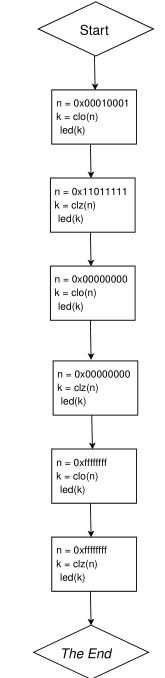
\includegraphics[scale=0.7]{../images/code_schema.png}
             \end{figure}
     \section*{Временные диаграммы}
        Сигналы:
        \begin{enumerate}
            \item result -- результат операции;
            \item b\_in  -- входной операнд, над которым производится операция;
            \item alu\_ctl -- код операции ( clo -- 11; clz -- 10).
        \end{enumerate}
        \begin{figure}[H]
            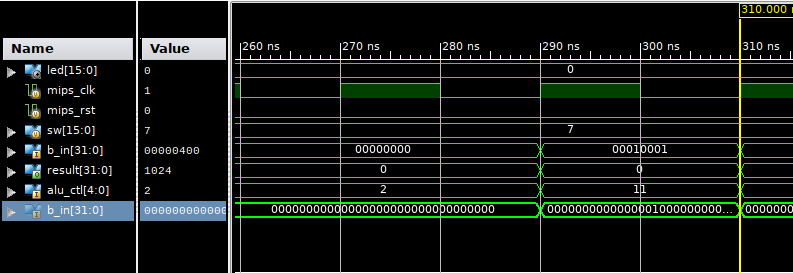
\includegraphics[scale=0.5]{../images/clo_1.png}
            \caption{Input: 0x00010001}
        \end{figure}
        \begin{figure}[H]
            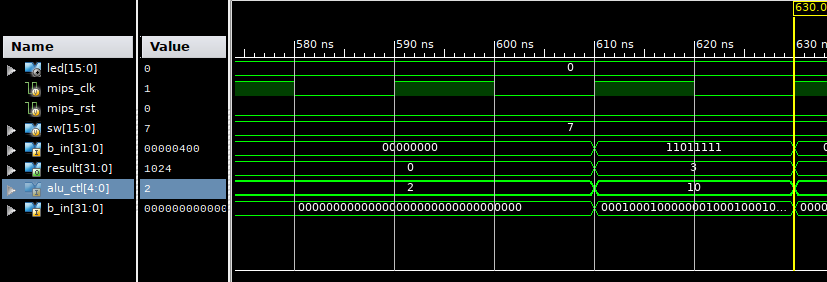
\includegraphics[scale=0.5]{../images/clz_1.png}
            \caption{Input: 0x11011111}
        \end{figure}

        \begin{figure}[H]
            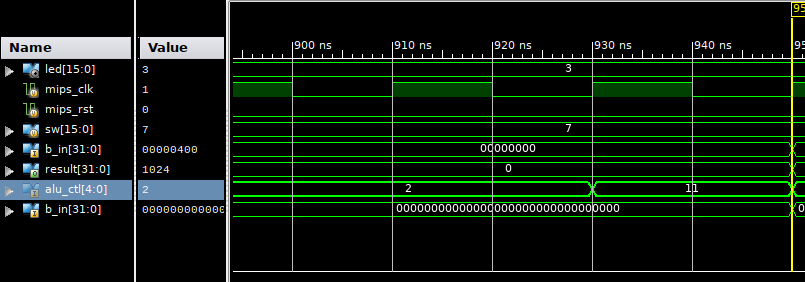
\includegraphics[scale=0.5]{../images/clo_2.png}
            \caption{Input: 0x00000000}
        \end{figure}
        \begin{figure}[H]
            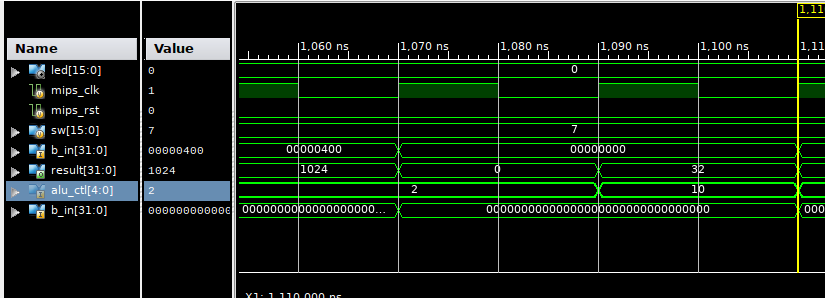
\includegraphics[scale=0.5]{../images/clz_2.png}
            \caption{Input: 0x00000000}
        \end{figure}

        \begin{figure}[H]
            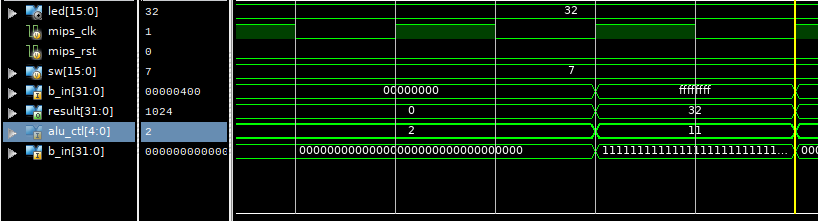
\includegraphics[scale=0.5]{../images/clo_3.png}
            \caption{Input: 0x11111111}
        \end{figure}
        \begin{figure}[H]
            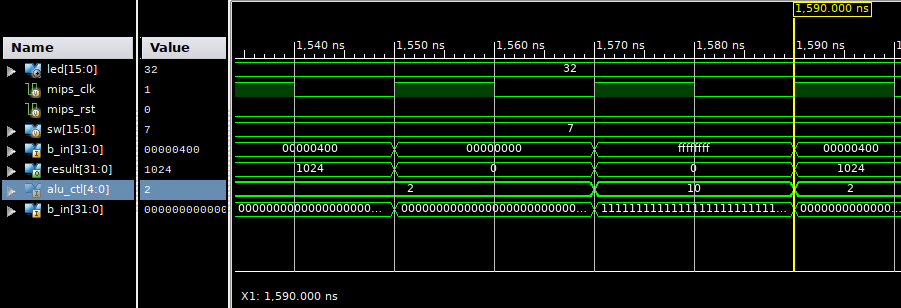
\includegraphics[scale=0.5]{../images/clz_3.png}
            \caption{Input: 0x11111111}
        \end{figure}

     \section*{Листинг}
        \lstinputlisting{../sw/test.asm}
        В файле alu.v.
        \lstinputlisting{../diff/alu.diff}
        В файле control.v.
        \lstinputlisting{../diff/control.diff}
    \section*{Вывод}
    В ходе выполнения лабораторной работы были добавлены команды clo (count
    leading ones) и clz (count leading zeros). Обнаружилось, что предлагаемый
    к работе компилятор работает с подмножеством ассемблера MIPS, который не
    содержит в себе данные команды, так что при написании и комплияции кода
    приходилось переводить команды в машинный код вручную. 
\end{document}
